\section{Cost-Based Optimization from Meta-Decompositions}
\label{sec:opt}

Even though we have presented an algorithm, enumerating all possible join trees is infeasible, as their number grows exponentially with the number of relations, as shown by \cref{thm:exp-join-trees}. Instead, we propose a cost-based optimization algorithm that \emph{operates directly on the meta-decomposition} to find an optimal width-1 query plan.  
Similar to the case for join tree enumeration discussed in \cref{sec:enum}, the search space for such plans is defined by four key factors: (1)~selecting a root of the join tree to induce the width-1 query plan; (2) unnesting minor nodes; (3) handling possible re-branching, and (4) determining the local join order for each node and its neighbors.  In this section, we detail our procedure to address them.  

\subsection{Re-Branching}

As previously discussed, re-branching can happen when a child node $c$ of a node $p$ in the meta-decomposition could also be a child of another descendant node $d$ of $p$ in a join tree, if $\kappa(c) \subsetneq \kappa(d)$.
This scenario, however, is in fact very rare in practice: we found no query in the JOB benchmark that exhibited this scenario, and only one query in the TPC-H benchmark can involve re-branching.
Therefore, for simplicity, we do not consider re-branching when describing the algorithm in this section. 
As we show in the \arxivorappendix, accommodating a possible re-branching adds only a constant factor to the overall complexity.

\begin{algorithm}[t]
\caption{Finding the optimal width-1 query plan to evaluate the query induced by a meta-decomposition}
\label{alg:cost}
\SetKwInOut{Input}{input}
\SetKwInOut{Output}{output}
\SetKwInOut{Known}{known}
\Input{A meta-decomposition $M = (V(M), r(M), E(M), \lambda, \chi, \kappa)$}
\Output{The optimal query plan}

\tcp*[l]{Bottom-up traversal}

\ForEach{non-root node $q \in V(M)$, in bottom-up order}{
    $p \gets$ $q$'s parent node on $M$\;
    $ {\sf plan}(T_{p \to q}) \gets {\sf optimizeLocal}(q, \set{{\sf plan}(T_{q \to c}) : c \in \mathsf{children}(q)})$ 
}

${\sf plan}(M) \gets {\sf optimizeLocal}(r, \set{ {\sf plan}(T_{r \to c}) : c \in \mathsf{children}(r) })$ \;

\tcp*[l]{Top-down traversal}

\ForEach{$c \in \mathsf{children}(r)$}{
    ${\sf plan}(T_{c \to r}) \gets {\sf optimizeLocal}(r, \set{{\sf plan}(T_{r \to c'}) : c' \in \mathsf{children}(r)\setminus \set{c}})$ \;
}

\ForEach{non-root node $q \in V(M)$, in top-down order}{
    $p \gets q$'s parent node on $M$\;
    \ForEach{child $c \in C(q)$} {
        ${\sf plan}(T_{c \to q}) \gets {\sf optimizeLocal}(q, \set{{\sf plan}(T_{q \to p})} \cup \set{{\sf plan}(T_{q \to c'}) : c' \in \mathsf{children}(r)\setminus \set{c}})$ \;
    }
}

\Return{the plan $
{\sf plan}(T_{p \to q}) \bowtie {\sf plan}(T_{q \to p})
$ with the minimum cost among all $(p, q) \in E(M)$ }

\end{algorithm}

\subsection{The Overall Algorithm}

Given a meta-decomposition $M$, our algorithm to produce a width-1 query plan is shown in \cref{alg:cost}. This algorithm first makes two traversals of $M$, one bottom-up and one top-down.

In the bottom-up traversal, for each non-root node $q$, we find the optimal plan to join the relation in $q$ and all the plans given by the children of $q$, which gives the optimal plan to evaluate $Q(T_q)$, the query induced by the subtree of $M$ rooted at $q$.

\begin{example}
    For the query $Q_{\ref{ex:hierarchical}}$ in \cref{ex:hierarchical}, with meta-decomposition shown in \cref{fig:hierarchical-meta}, this bottom-up traversal visits the nodes in the following order. 
    (For simplicity, we simply use $R_i$ to refer to the node with $\lambda$-label $\{ R_i \}$.)
    \begin{enumerate}[leftmargin=*]
        \item $R_3$. It generates the plan for the subtree $T_{R_3}$, or $T_{R_2 \rightarrow R_3}$, containing $R_3$ only. The plan is simply a scan of $R_3$.
        \item $R_2$. It generates the plan for $T_{R_2}$, or $T_{R_1 \rightarrow R_2}$, containing $R_2$ and $R_3$. It simply needs to join $R_2$ with the plan for $T_{R_3}$ in the previous step, i.e., $R_2 \bowtie R_3$.
        \item $R_4$. It generates the plan for the subtree $T_{R_4}$, or $T_{R_1 \rightarrow R_4}$, containing $R_4$ only. The plan is simply a scan of $R_4$.
        \item $R_1$. This is the root node. The traversal terminates here.
    \end{enumerate}
\end{example}

Then, in the top-down traversal, for each node $q$ and each child $c$ of $q$ on the meta-decomposition, we find the optimal plan to join $q$ and all plans given by the neighbors (parent and children) of $q$ except $c$, which gives the optimal plan to join all relations in $T_{c \to q}$.

\begin{example}
    Again for $Q_{\ref{ex:hierarchical}}$, the top-down traversal visits the nodes in the following order.
    \begin{enumerate}[leftmargin=*]
        \item $R_1 \to$ child $R_2$. It generates the plan for the subtree $T_{R_2 \rightarrow R_1}$, containing $R_1$ and $R_4$. The plan is simply $R_1 \bowtie R_4$.
        \item $R_2 \to$ child $R_3$. It generates the plan for the subtree $T_{R_3 \rightarrow R_2}$, containing $R_1$, $R_2$, and $R_4$. Similarly, we join $R_2$ with the result of $R_1 \bowtie R_4$, which is the plan for the subtree $T_{R_2 \rightarrow R_1}$.
        \item $R_1 \to$ child $R_4$. It generates the plan for the subtree $T_{R_4 \rightarrow R_1}$, containing $R_1$, $R_2$, and $R_3$. Here, $R_2$ and $R_3$ are in the same subtree $T_{R_1 \rightarrow R_2}$ of $R_1$. So, we first take the plan generated for this subtree, which is $R_2 \bowtie R_3$, and then join this result with $R_1$.
    \end{enumerate}
\end{example}

At the end, we choose the root of the query plan, which is the minimum-cost plan of the form ${\sf plan}(T_{p \to q}) \bowtie {\sf plan}(T_{q \to p})$ among all $(p, q) \in E(M)$. For example, the width-1 plan shown in \cref{fig:hierarchical-plan} corresponds to ${\sf plan}(T_{R_2 \to R_1}) \bowtie {\sf plan}(T_{R_1 \to R_2})$.

In the example we just considered, the fan-out is 2. For higher fan-outs, at each node in the meta-decomposition, we need to decide on an order to join the results of multiple subtrees. To do so, the algorithm calls the function $\sf optimizeLocal $, which optimizes the local join for each node and its neighbors. We will elaborate on this in \cref{sec:local-join}. 




\subsection{Optimizing the Local Join with Neighbors}
\label{sec:local-join}
One essential component of this algorithm is to, for a vertex $q$ in the meta-decomposition, find the optimal plan to join the relation in this vertex and the optimal query plans given by (a subset of) its neighbors ($\sf optimizeLocal$).  This can be viewed as a classic star join optimization problem, where $R_q$ is the hub relation, and the result of the induced query $Q(T_{c_i})$ from each of its neighbors $c_i$ is a satellite relation, denoted by $R_{i}$ for $i = 1, \dots, f(q)$, where $\chi(c_i) \cap \chi(q) \neq \emptyset$ and $\chi(c_i) \cap \chi(c_j) \subseteq \chi(q)$ for all $i \neq j$.
Unfortunately, even in this restricted setting, this problem of optimizing the join of $R_q$ and all $R_i$'s is still \NP{}-hard, because this can be reduced from the problem of optimizing the ordering of a Cartesian product $S_1 \times S_2 \times \cdots \times S_n$---which is already shown to be \NP{}-hard \cite{scheufele_constructing_1996}---by adding a shared attribute to each $S_i$ such that all tuples have the same value for this attribute.  By using dynamic programming algorithms~\cite{moerkotte_dynamic_2008,stoian_dpconv_2024}, the problem can be solved in $\widetilde{O}(2^{f(q)} \cdot (f(q))^3)$
, where $\widetilde{O}$ suppresses poly-logarithmic factors, and the fan-out $f(q)$ is the number of children of $q$ on the meta-decomposition.  However, as mentioned in Section~\ref{sec:hierarchical-query-plan}, \emph{the fan-out of real-world queries is typically very small}. This makes the exponential-time exact algorithm practical for the vast majority of cases. 
In the rare case that a node has a high fan-out, making the exact DP algorithm too slow, we can substitute it with a heuristic. An effective choice is Greedy Operator Ordering~(GOO)~\cite{fegaras_new_1998}, which iteratively joins the neighbor that results in the smallest intermediate result. This method is outlined in the \arxivorappendix.

\subsection{Case Study: Optimizing Relation-Dominated Queries with Meta-Decompositions}

Our framework naturally incorporates projection pushdown for early cardinality reduction. When building a plan for a subquery, such as $\textsf{plan}(T_{p \to q})$ in \cref{alg:cost}, we can immediately project the result to only the attributes needed for subsequent operations.
Specifically, after computing the joins within the subtree $T_q$, we only need to retain (1)~attributes that are part of the final output, and
(2)~attributes required for joining with the remaining relations, which is $\kappa(q)$ by definition.

This strategy is especially effective for relation-dominated queries, where a single relation contains all output attributes.  If a subtree contains no output attributes, we can project its result to only $\kappa(q)$, i.e., the join keys with the remaining relations, which can significantly reduce the size of intermediate results.
However, traditional dynamic-programming-based optimizers lack such a comprehensive structural view. Therefore, they typically do not identify such opportunities and must consider the entire search space of query plans, relying solely on cost estimation.

\begin{example} \label{ex:rel-dom}
\begin{figure}
    \centering
    \small
    \hfill
    \begin{subfigure}{.5\linewidth}
        \centering
        \vspace{-0.5\baselineskip}
        \begin{tikzpicture}[hypergraph,xscale=.75,yscale=0.7,trim left=0cm,trim right=0cm]
            \node[vertex,label={west:$x_{\sf mid}$}] (mid) at (0, 0) {};
            \node[vertex,label={east:$x_{\sf kid}$}] (kid) at (-2.5, 0) {};
            \node[vertex,label={east:$x_{\sf k}$}] (k) at (-4, 0) {};

            \node[vertex,label={east:$x_{\sf pid}$}] (pid) at (0, -1.5) {};
            \node[vertex,label={east:$x_{\sf n}$}] (n) at (0, -2.5) {};
            
            \node[vertex,label={west:$x_{\sf cid}$}] (cid) at (2.5, 0) {};
            \node[vertex,label={west:$x_{\sf cc}$}] (cc) at (4, 0) {};
            
            \node[vertex,label={west:$x_{\sf t}$}] (t) at (0, 1) {};
        
            \begin{scope}[on background layer]
                    
                
                \newcommand*{\patht}{($(t) + (0,0.5)$)
        					to[out=180,in=180] ($(mid) + (0,-0.5)$)
        					to[out=0,in=0] ($(t) + (0,0.5)$)}

                \newcommand*{\pathmk}{	($(mid) + (0.25,0.25)$)
                    to[out=135,in=135] ($(kid) + (-0.25,-0.25)$)
                    to[out=-45,in=-45] ($(mid) + (0.25,0.25)$)}
                
                \newcommand*{\pathk}{($(kid) + (0.6,0)$)
        					to[out=90,in=90] ($(k) + (-0.5,0)$)
        					to[out=-90,in=-90] ($(kid) + (0.6,0)$)}

                \newcommand*{\pathci}{($(mid) + (0,0.5)$)
        					to[out=180,in=180] ($(pid) + (0,-0.5)$)
        					to[out=0,in=0] ($(mid) + (0,0.5)$)}

                \newcommand*{\pathn}{($(pid) + (0,0.5)$)
        					to[out=180,in=180] ($(n) + (0,-0.5)$)
        					to[out=0,in=0] ($(pid) + (0,0.5)$)}
                
                \newcommand*{\pathmc}{($(mid) + (-0.25,0.25)$)
                    to[out=45,in=45] ($(cid) + (0.25,-0.25)$)
                    to[out=-135,in=-135] ($(mid) + (-0.25,0.25)$)}
                
                \newcommand*{\pathcn}{($(cid) + (-0.5,0)$)
        					to[out=90,in=90] ($(cc) + (0.5,0)$)
        					to[out=-90,in=-90] ($(cid) + (-0.5,0)$)}
                
                \draw[hyperedge,looseness=1,draw=Red,fill=Red,fill opacity=.1] \patht;
                \draw[hyperedge,looseness=1,draw=Fuchsia,fill=Fuchsia,fill opacity=.1] \pathmk;
                \draw[hyperedge,looseness=1,draw=NavyBlue,fill=NavyBlue,fill opacity=.1] \pathk;
                \draw[hyperedge,looseness=1, draw=BurntOrange,fill=BurntOrange,fill opacity=.1] \pathmc;
                \draw[hyperedge,looseness=1, draw=TealBlue,fill=TealBlue,fill opacity=.1] \pathcn;
                \draw[hyperedge,looseness=1, draw=Gray,fill=Gray,fill opacity=.1] \pathci;
                \draw[hyperedge,looseness=1, draw=Thistle,fill=Thistle,fill opacity=.1] \pathn;
        
                \node[text=Red] at (0.75,1.25) {$R_{\sf t}$};
                \node[text=Fuchsia] at (-1.5,1) {$R_{\sf mk}$};
                \node[text=Cyan] at (-3.25,1) {$R_{\sf k}$};
                \node[text=BurntOrange] at (1.6,1) {$R_{\sf mc}$};
                \node[text=TealBlue] at (3.25,1) {$R_{\sf cn}$};
                \node[text=Gray] at (-1,-1) {$R_{\sf ci}$};
                \node[text=Thistle] at (-1,-2.25) {$R_{\sf n}$};
                
            \end{scope}
        \end{tikzpicture}
        \caption{Hypergraph}
        \label{fig:rel-dom-hg}
    \end{subfigure}
    \hfill
    \begin{subfigure}{.33\linewidth}
        \centering
        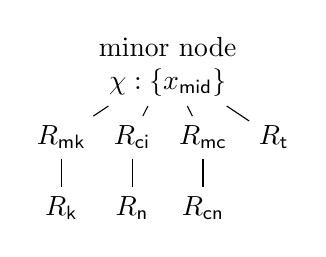
\begin{tikzpicture}[
			level distance=0.9cm,
			level 1/.style={sibling distance=0.9cm}
        ]
			\node[align=center] { minor node \\ $\chi: \{ x_{\sf mid} \}$ }
				child { node {$R_{\sf mk}$} edge from parent[-]
                    child { node {$R_{\sf k}$} edge from parent[-] }
                }
                child { node {$R_{\sf ci}$} edge from parent[-]
                    child { node {$R_{\sf n}$} edge from parent[-] }
                }
                child { node {$R_{\sf mc}$} edge from parent[-]
                    child { node {$R_{\sf cn}$} edge from parent[-] }
                }
                child { node {$R_{\sf t}$} edge from parent[-] };
                
		\end{tikzpicture}
        \caption{Meta-decomposition (simplified)}
        \label{fig:rel-dom-meta}
    \end{subfigure}
    \hfill \ 

    \begin{subfigure}{.3\linewidth}
        \centering
        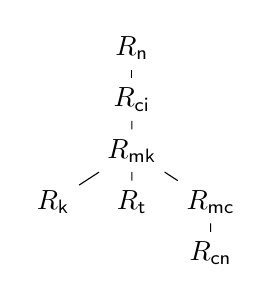
\begin{tikzpicture}[
			level distance=0.65cm,
			level 1/.style={sibling distance=1cm}
        ]
			\node { $R_{\sf n}$ }
				child { node {$R_{\sf ci}$} edge from parent[-]
                    child { node {$R_{\sf mk}$} edge from parent[-]
                        child { node {$R_{\sf k}$} edge from parent[-] }
                        child { node {$R_{\sf t}$} edge from parent[-] }
                        child { node {$R_{\sf mc}$} edge from parent[-]
                            child { node {$R_{\sf cn}$} edge from parent[-] }
                        }
                    }
                };
                
		\end{tikzpicture}
        \caption{Join tree inducing the width-1 plan in \cref{fig:rel-dom-w1}}
        \label{fig:rel-dom-jt}
    \end{subfigure}
    \hfill
    \begin{subfigure}{.33\linewidth}
        \centering
        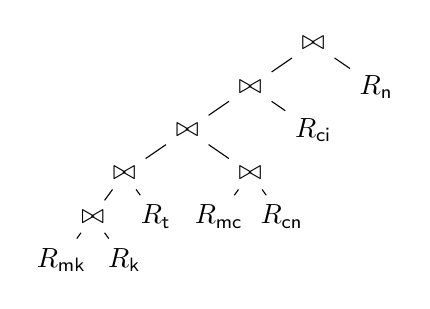
\begin{tikzpicture}[
			level distance=0.55cm,
            level 1/.style={sibling distance=1.6cm},
			level 2/.style={sibling distance=1.6cm},
            level 3/.style={sibling distance=1.6cm},
            level 4/.style={sibling distance=0.8cm}
        ]
			\node { $\bowtie$ }
                child { node {$\bowtie$} edge from parent[-]
                    child { node {$\bowtie$} edge from parent[-]
                        child { node {$\bowtie$} edge from parent[-]
            				child { node {$\bowtie$} edge from parent[-]
                                child { node {$R_{\sf mk}$} edge from parent[-] }
                                child { node {$R_{\sf k}$} edge from parent[-] }
                            }
                            child { node {$R_{\sf t}$} edge from parent[-] }
                        }
                        child { node {$\bowtie$} edge from parent[-]
                            child { node {$R_{\sf mc}$} edge from parent[-] }
                            child { node {$R_{\sf cn}$} edge from parent[-] }
                        }
                    }
                    child { node {$R_{\sf ci}$} edge from parent[-] } 
                }
                child { node {$R_{\sf n}$} edge from parent[-] };
		\end{tikzpicture}
        \caption{Optimal width-1 query plan, induced by the join tree in \cref{fig:rel-dom-jt}}
        \label{fig:rel-dom-w1}
    \end{subfigure}
    \hfill
    \begin{subfigure}{.3\linewidth}
        \centering
        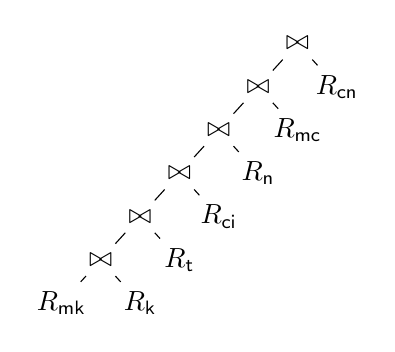
\begin{tikzpicture}[
			level distance=0.55cm,
			level 1/.style={sibling distance=1cm}
        ]
			\node { $\bowtie$ }
                child { node {$\bowtie$} edge from parent[-]
                    child { node {$\bowtie$} edge from parent[-]
                        child { node {$\bowtie$} edge from parent[-]
            				child { node {$\bowtie$} edge from parent[-]
                				child { node {$\bowtie$} edge from parent[-]
                                    child { node {$R_{\sf mk}$} edge from parent[-] }
                                    child { node {$R_{\sf k}$} edge from parent[-] }
                                }
                                child { node {$R_{\sf t}$} edge from parent[-] }
                            }
                            child { node {$R_{\sf ci}$} edge from parent[-] }
                        }
                        child { node {$R_{\sf n}$} edge from parent[-] }
                    }
                    child { node {$R_{\sf mc}$} edge from parent[-] }
                }
                child { node {$R_{\sf cn}$} edge from parent[-] };
		\end{tikzpicture}
        \caption{Optimal plan by dynamic programming, of width 2}
        \label{fig:rel-dom-duckdb}
    \end{subfigure}
    % \vspace{-0.75\baselineskip}
    \caption{The hypergraph, the meta-decomposition, the optimal width-1 query plan with the inducing join tree, and the optimal query plan (of width 2) found by dynamic programming, of the query JOB 17f in \cref{ex:rel-dom}}
    \label{fig:rel-dom}
\end{figure}

    Take query 17f in the join order benchmark~(JOB) as an example. Omitting irrelevant attributes in each relation, this query can be abstractly represented as
    \begin{align*}
        Q_{\ref{ex:rel-dom}} \gets \pi_{x_{\rm n}} ( 
            & R_{\sf ci}[x_{\sf mid}, x_{\sf pid}] \bowtie R_{\sf cn}[x_{\sf cid}, x_{\sf cc}] \bowtie \sigma_{x_{\sf k} = \cdots}(R_{\sf k}[x_{\sf kid}, x_{\sf k}])
            \bowtie R_{\sf mc}[x_{\sf mid}, x_{\sf cid}] \\
            & \bowtie R_{\sf mk}[x_{\sf mid}, x_{\sf kid}] \bowtie \sigma_{x_{\sf n} = \cdots}(R_{\sf n}[x_{\sf pid}, x_{\sf n}]) \bowtie R_{\sf t}[x_{\sf mid}, x_{\sf t}] 
        ).
    \end{align*}
    This is a relation-dominated query, as it has only one output attribute $x_{\sf n}$, which is an attribute of $R_{\sf n}$.
    \cref{fig:rel-dom} shows the hypergraph, the optimal width-1 query plan (found by \sys{} given cardinalities of the real data set), along with the join tree inducing it, and a width-2 query plan (which is the plan given by dynamic programming).
    In the width-1 plan in \cref{fig:rel-dom-w1}, \emph{all intermediate join results can be projected to a single attribute}, since the interface is always only one attribute, and there is no output attribute before the final join with $R_{\sf n}$.
    But, with the width-2 query plan in \cref{fig:rel-dom-duckdb}, \emph{the result of $((R_{\sf mk} \bowtie R_{\sf k}) \bowtie R_{\sf t}) \bowtie R_{\sf ci}$ has to be projected to two attributes $x_{\sf mid}$ and $x_{\sf pid}$}, which are join keys with $R_{\sf mc}$ and $R_{\sf n}$, respectively.
    Executing these plans, we indeed observe that \emph{the width-1 plan has a {\rm 1.72x} speedup over the width-2 plan}.
\end{example}

As with evaluating select-project-join queries, one can easily modify the cost model and use a join tree–based query evaluation algorithm, including any Yannakakis-style algorithm, that incorporates cost-based optimization via meta-decompositions. We hope this work inspires further research in related areas and encourages the integration of these theoretically desirable query evaluation techniques into practical systems.

